%!TEX root = ../../../super_main.tex

\section{Android GUI thread}
\label{sec:gui_thread_async_task}

The Android system imposes real time constraints on applications to keep them smooth and lag free. This section covers how we make sure we do not violate these constraints across all application code.

\section{GUI thread}
The real time constraints are implemented on a special GUI thread which runs the user interface event loop, which is basicly a queue of lesser tasks. Applications, e.g. activities, in the Android eco system runs, i.e updates their views, on this GUI thread. Any updates to views not coming from the GUI thread will result in an exception. This makes it easy to implement real time constraints on the GUI thread by simply setting a hard limit on how long, in real time, lesser tasks on the GUI thread are allowed to run. Any violation of the constraints will result in an Application Not Responding (ANR) message to the user \parencite{android_avoid_anr}. Users will not be able to distinguish an unresponsive application, e.g. the result of a deadlock, from a task taking too long on the GUI thread which may cause the user to terminate an otherwise functioning Application that was doing some complicated database query or downloading some file from the Internet. 

\section{The solution: AsyncTask}

The Android framework provides a very useful abstraction which makes it easy to run long tasks in the background with a class called AsyncTask. The AsyncTask provides 4 non final methods that makes it easy to synchronize between a background thread and the GUI thread. The three methods \androidinline{onPreExecute}, \androidinline{onProgressUpdate}, \androidinline{onPostExecute} are always all guaranteed to run on the GUI thread. While the last method \androidinline{doInBackground} always runs on an unspecified background thread from a pool of threads maintained by the system. The class then ensures an order on these method calls being: \androidinline{onPreExecute}, \androidinline{doInBackground}, \androidinline{onPostExecute}. The \androidinline{onProgressUpdate} method can be run multiple times while the doInBackground method is running and is started by a call to a method called \androidinline{publishProgress} from the \androidinline{doInBackground} method.  

\section{Long tasks}

Not causing the application to show an ANR message is one thing, making the user explicitly aware that a longer task is running, through some kind of feedback, is considered good practice \parencite{benyon}. We have tried to provide this feedback through Android \androidinline{ProgressBar} widgets whenever longer operation take place. The name ``ProgressBar'' is a bit misleading since the style of the \androidinline{ProgressBar} we use, which is the default style, is more like a spinning activity indicator as seen in \figref{fig:activity_indicator}. 

\begin{figure}[!htbp]
        \centering
        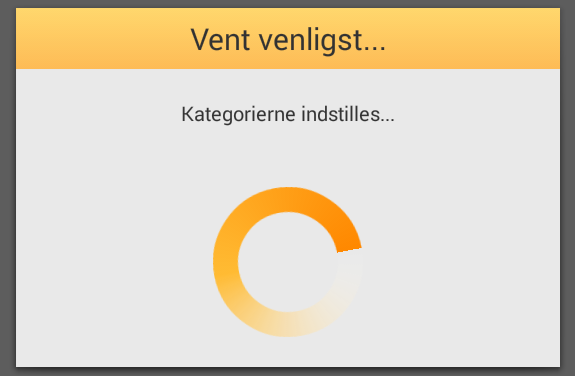
\includegraphics[width=0.75\textwidth]{sprint_three/progressbar_example}
        \caption{Android ProgressBar as an activity indicator}
        \label{fig:activity_indicator}
\end{figure}